\documentclass[border=5pt]{standalone}

% Required for Bengali text rendering and math symbols
\usepackage{fontspec}
\usepackage{amsmath}
\usepackage{tikz}

\setmainfont{Noto Sans Bengali}

\begin{document}

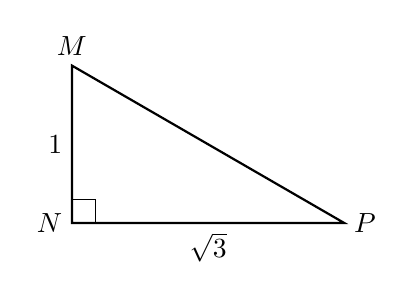
\begin{tikzpicture}[scale=1]

    % Define the coordinates based on 1 : sqrt(3) ratio
    \coordinate (N) at (0,0);
    \coordinate (M) at (0,2);
    \coordinate (P) at (3.46,0); % 2 * 1.732 (sqrt 3)

    % Draw the main triangle segments
    \draw[thick] (M) -- (N) -- (P) -- cycle;

    % Draw the right angle symbol at N
    \draw (0,0.3) -- (0.3,0.3) -- (0.3,0);

    % Label the vertices using Math Mode ($...$) to ensure visibility
    \node[left] at (N) {$N$};
    \node[above] at (M) {$M$};
    \node[right] at (P) {$P$};

    % Add measurements/labels exactly as shown in the image
    \node[left] at (0, 1) {$1$};
    \node[below] at (1.73, 0) {$\sqrt{3}$};

\end{tikzpicture}

\end{document}
